\documentclass[11pt]{article}
\usepackage[utf8]{inputenc} % Para caracteres en espa�ol
\usepackage{amsmath,amsthm,amsfonts,amssymb,amscd}
\usepackage{multirow,booktabs}
\usepackage[table]{xcolor}
\usepackage{fullpage}
\usepackage{lastpage}
\usepackage{enumitem}
\usepackage{multicol}
\usepackage{fancyhdr}
\usepackage{mathrsfs}
\usepackage{pdfpages}
\usepackage{wrapfig}
\usepackage{setspace}
\usepackage{esvect}
\usepackage{calc}
\usepackage{multicol}
\usepackage{cancel}
\usepackage{graphicx}
\graphicspath{ {} }
\usepackage[retainorgcmds]{IEEEtrantools}
\usepackage[margin=3cm]{geometry}
\usepackage{amsmath}
\newlength{\tabcont}
\setlength{\parindent}{0.0in}
\setlength{\parskip}{0.05in}
\usepackage{empheq}
\usepackage{framed}
\usepackage[most]{tcolorbox}
\usepackage{xcolor}
\colorlet{shadecolor}{orange!15}
\parindent 0in
\parskip 12pt
\geometry{margin=1in, headsep=0.25in}
\theoremstyle{definition}
\newtheorem{defn}{Definition}
\newtheorem{reg}{Rule}
\newtheorem{exer}{Exercise}

% Two more packages that make it easy to show MATLAB code
\usepackage[T1]{fontenc}
\usepackage[framed,numbered]{matlab-prettifier}
\lstset{
	style = Matlab-editor,
	basicstyle=\mlttfamily\small,
}

\newtheorem{note}{Note}
\begin{document}
\begin{lstlisting}
function hw6_prob1
%% Problem 1 Part D
wn = [10^-2 10^-1 10^0 10^1 10^2];
J = 10; 		Jw = 1;  
A = [0 1; 0 0]; 	B = [0; 1/J];
x0 = [0.1; 0]; 		v0 = 0;
for j=1:length(wn)
    tRate = 30;
    tMax = 1;
    t = linspace(0,tMax,tMax*tRate);
    k = [wn(j)^2*J 2*J/sqrt(2)*wn(j)];
    for i=1:length(t)
        x(:,i) = expm((A-B*k)*t(i))*x0;
    end
    for i=1:length(t)
        v(:,i) = -k*(1/Jw)*inv(A-B*k)*(expm((A-B*k)*t(i))-eye(2))*x0;
    end
    theta(:,j) = x(1,:);
    uu(:,j)=-k*x;
    vv(:,j)=v;
end
    figure(1)
    subplot(3,1,1)
    subplot(3,1,2)
    plot(t,uu,'linewidth',2)
    subplot(3,1,3)
    plot(t,vv,'linewidth',2)
    
%% Problem 1 Part E
J = 10; 		Jw = 1;
A = [0 1; 0 0]; 	B = [0; 1/J]; 
x0 = [0.1; 0]; 		v0 = 0;
Q = eye(2); 		R = [10^-2 10^-1 10^0 10^1 10^2];
for j=1:length(R)
    t = linspace(0,10,1400);
    k = lqr(A,B,Q,R(j));
    for i=1:length(t)
        x(:,i) = expm((A-B*k)*t(i))*x0;
    end
    for i=1:length(t)
        v(:,i) = -k*(1/Jw)*inv(A-B*k)*(expm((A-B*k)*t(i))-eye(2))*x0;
    end
    thetae(:,j) = x(1,:);
    uue(:,j)=-k*x;
    vve(:,j)=v;
end 
    figure(2)
    subplot(3,1,1)
    plot(t,thetae,'linewidth',2)
    subplot(3,1,2)
    plot(t,uue,'linewidth',2)
    subplot(3,1,3)
    plot(t,vve)
\end{lstlisting}
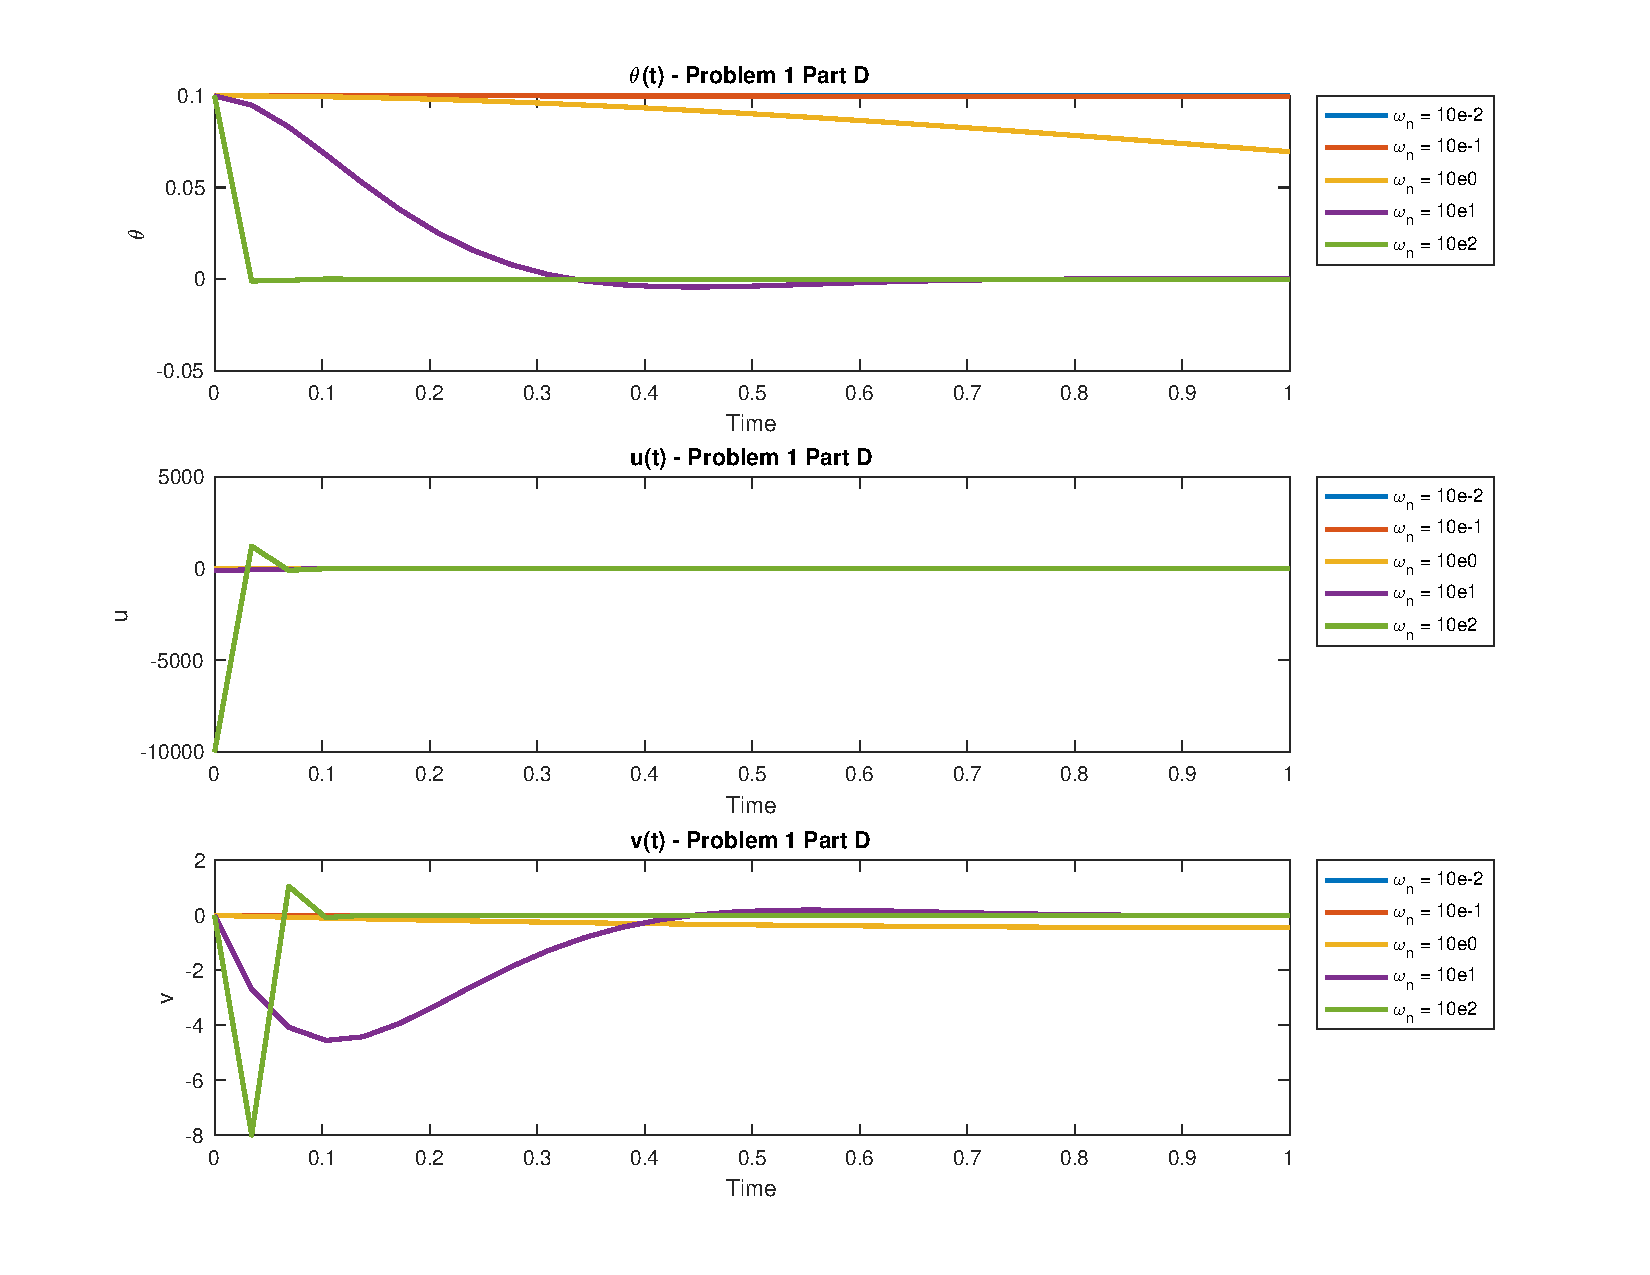
\includepdf{HW6P1D.pdf}
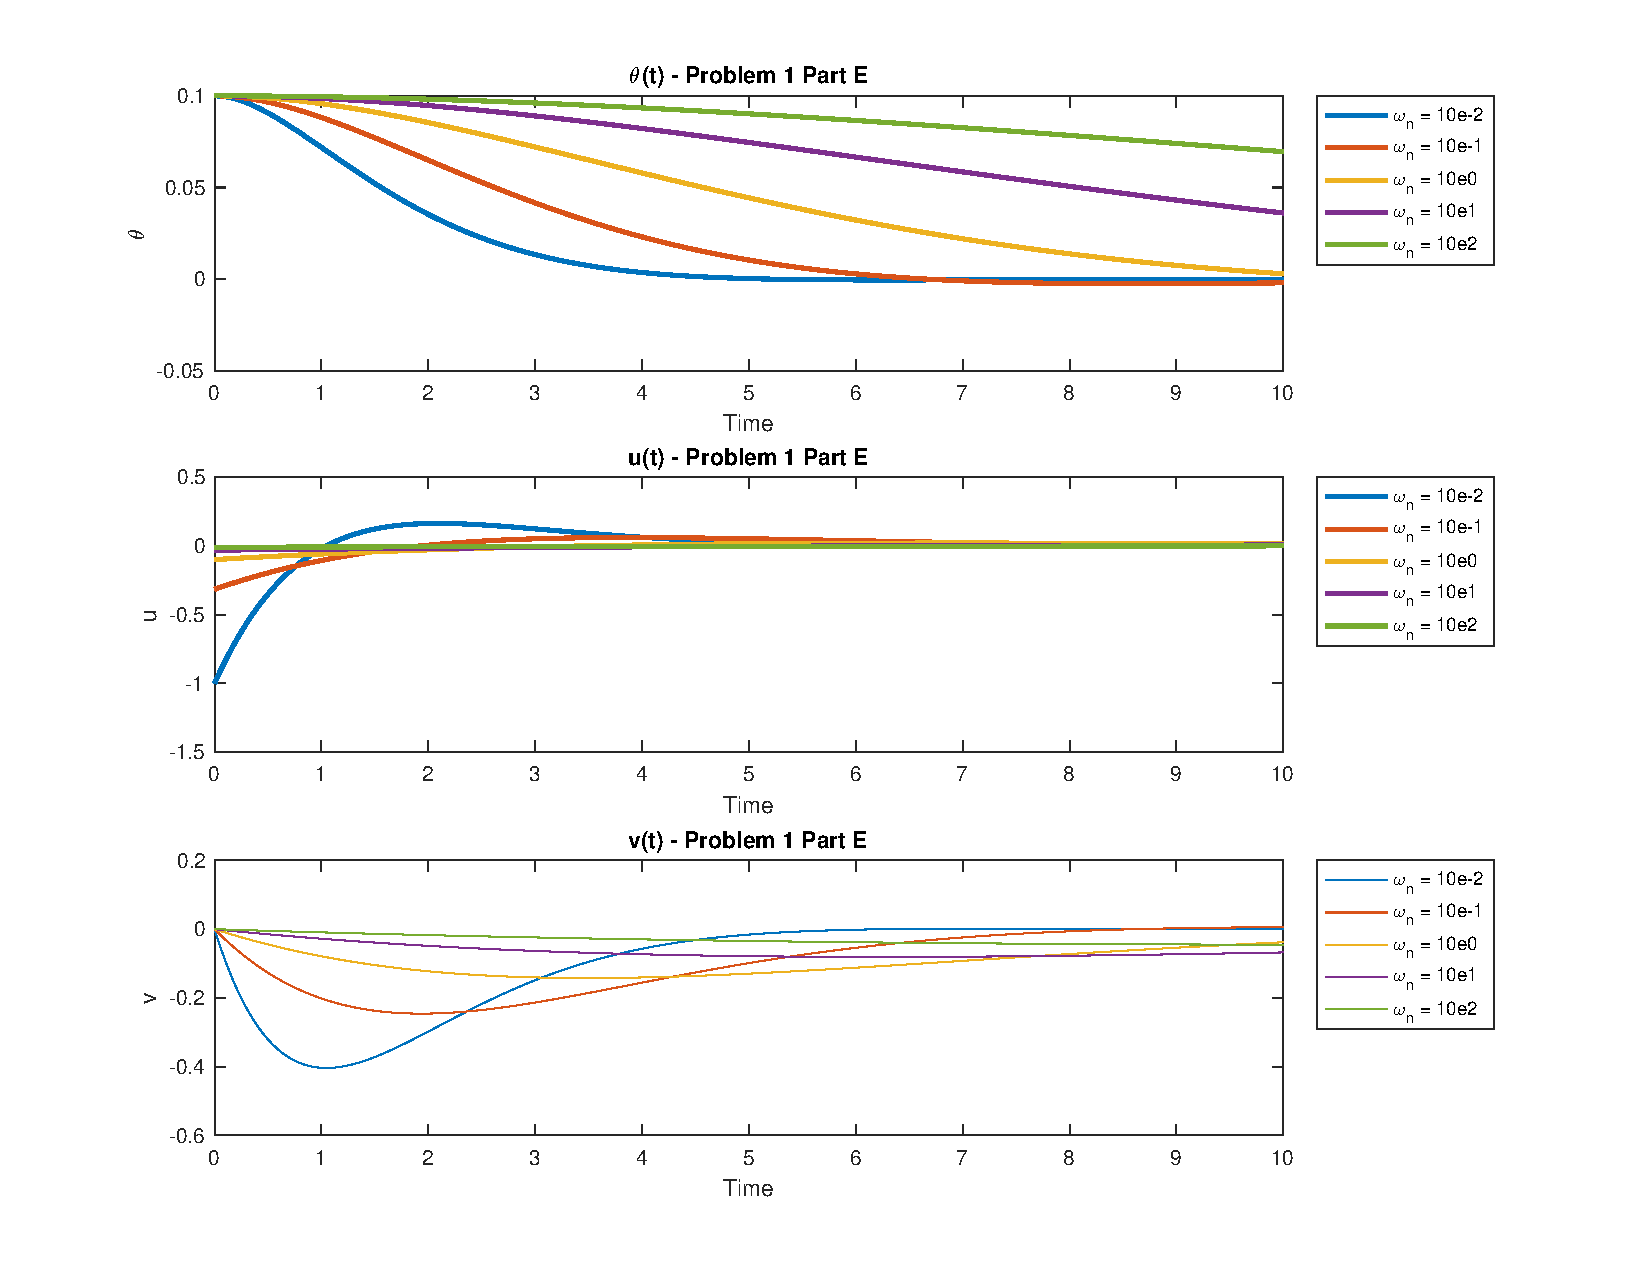
\includepdf{HW6P1E.pdf}

\begin{lstlisting}
function hw6p2t2
%% theta(t) v(t) and u(t) 2
J1 = 12;
J2 = 14;
J3 = 8; 
Jw = 1; 
n = .0011;

A = [0 1 0; 3*n^2*(J3-J1)/J2 0 0; 0 0 0];
B = [0; 1/J2; -1/Jw];
x0 = [0.5; 0; 0];

Q = eye(3);
R = 10^0; 

t = linspace(0,160,300);

% Part B Solution
[K,S,E] = lqr(A,B,Q,R)

for i=1:length(t)
    x(:,i) = expm((A-B*K)*t(i))*x0;
end

figure(1)
subplot(1,3,1)
plot(t,x(1,:));
subplot(1,3,2)
plot(t,x(2,:));
subplot(1,3,3)
plot(t,x(3,:));


figure(2)
plot(t,x, 'linewidth',2);

\end{lstlisting}
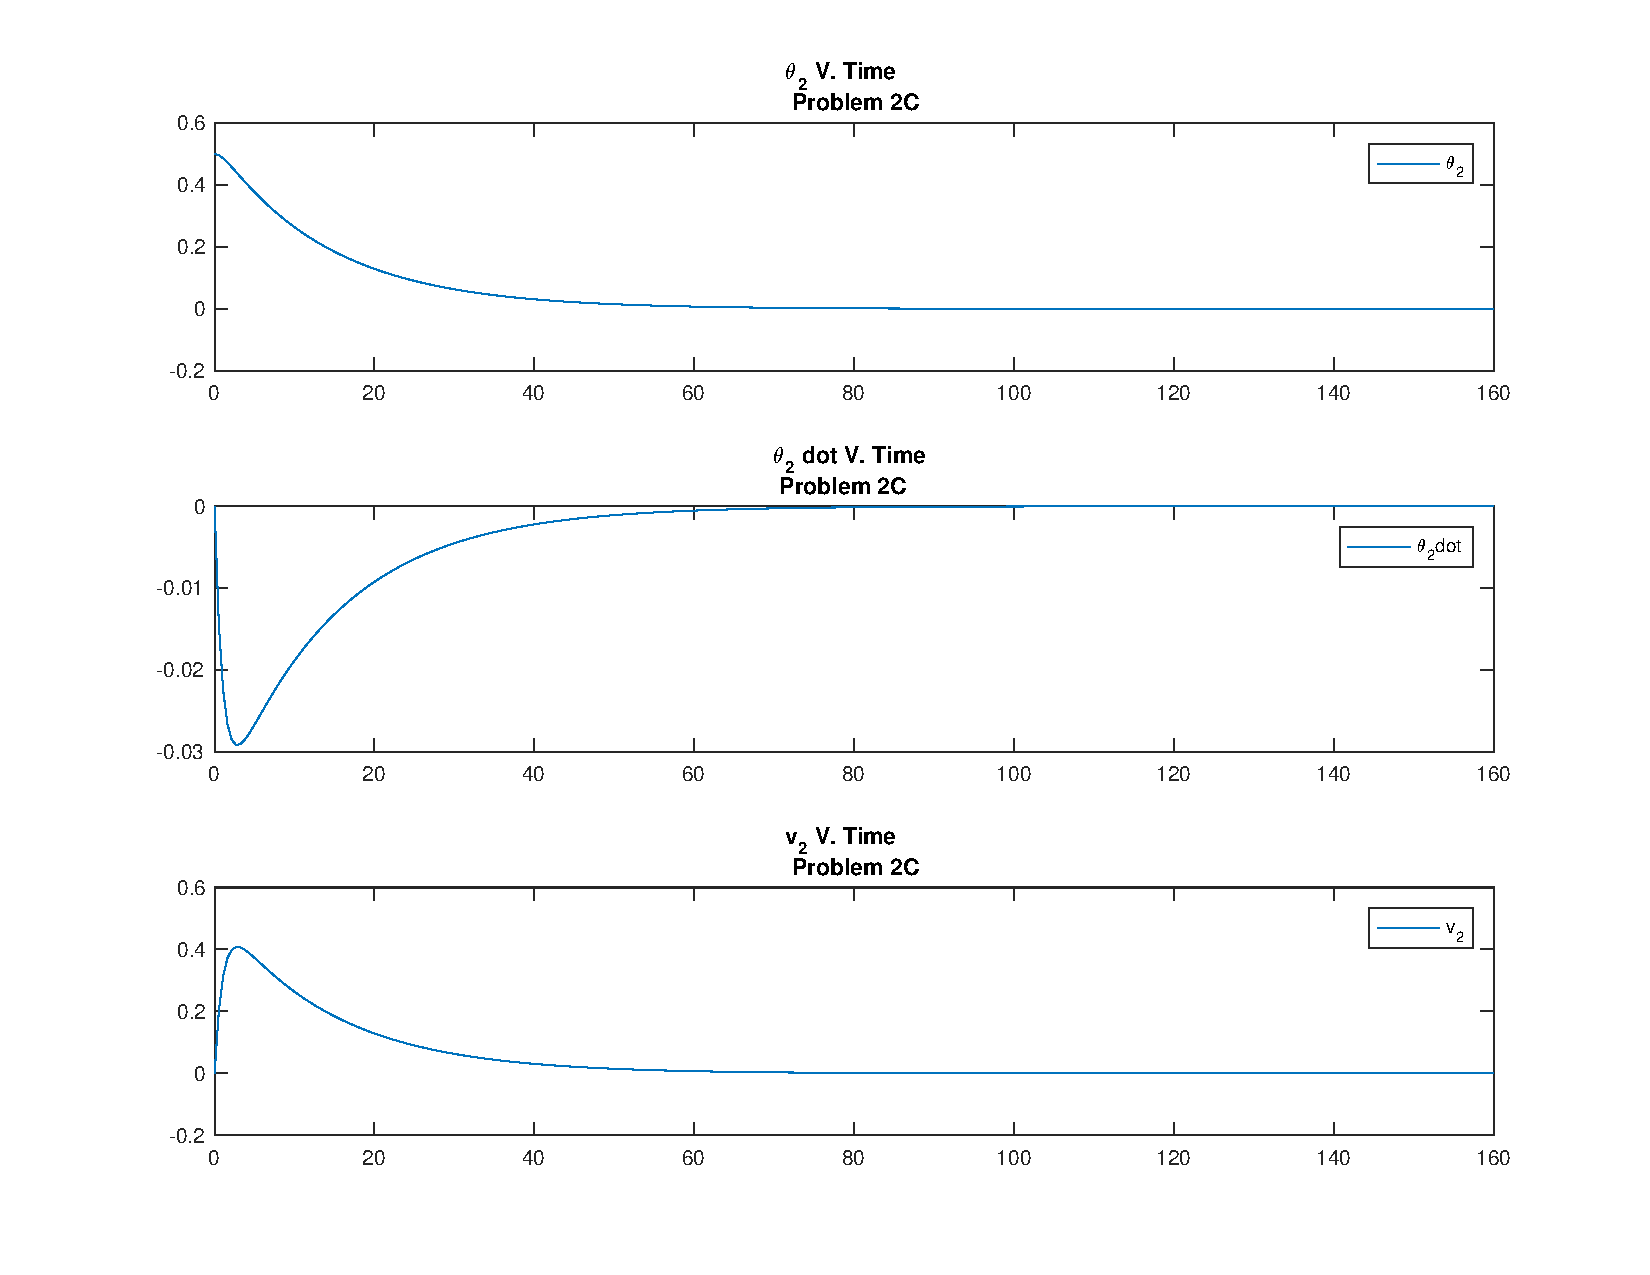
\includepdf{HW6P2C1.pdf}
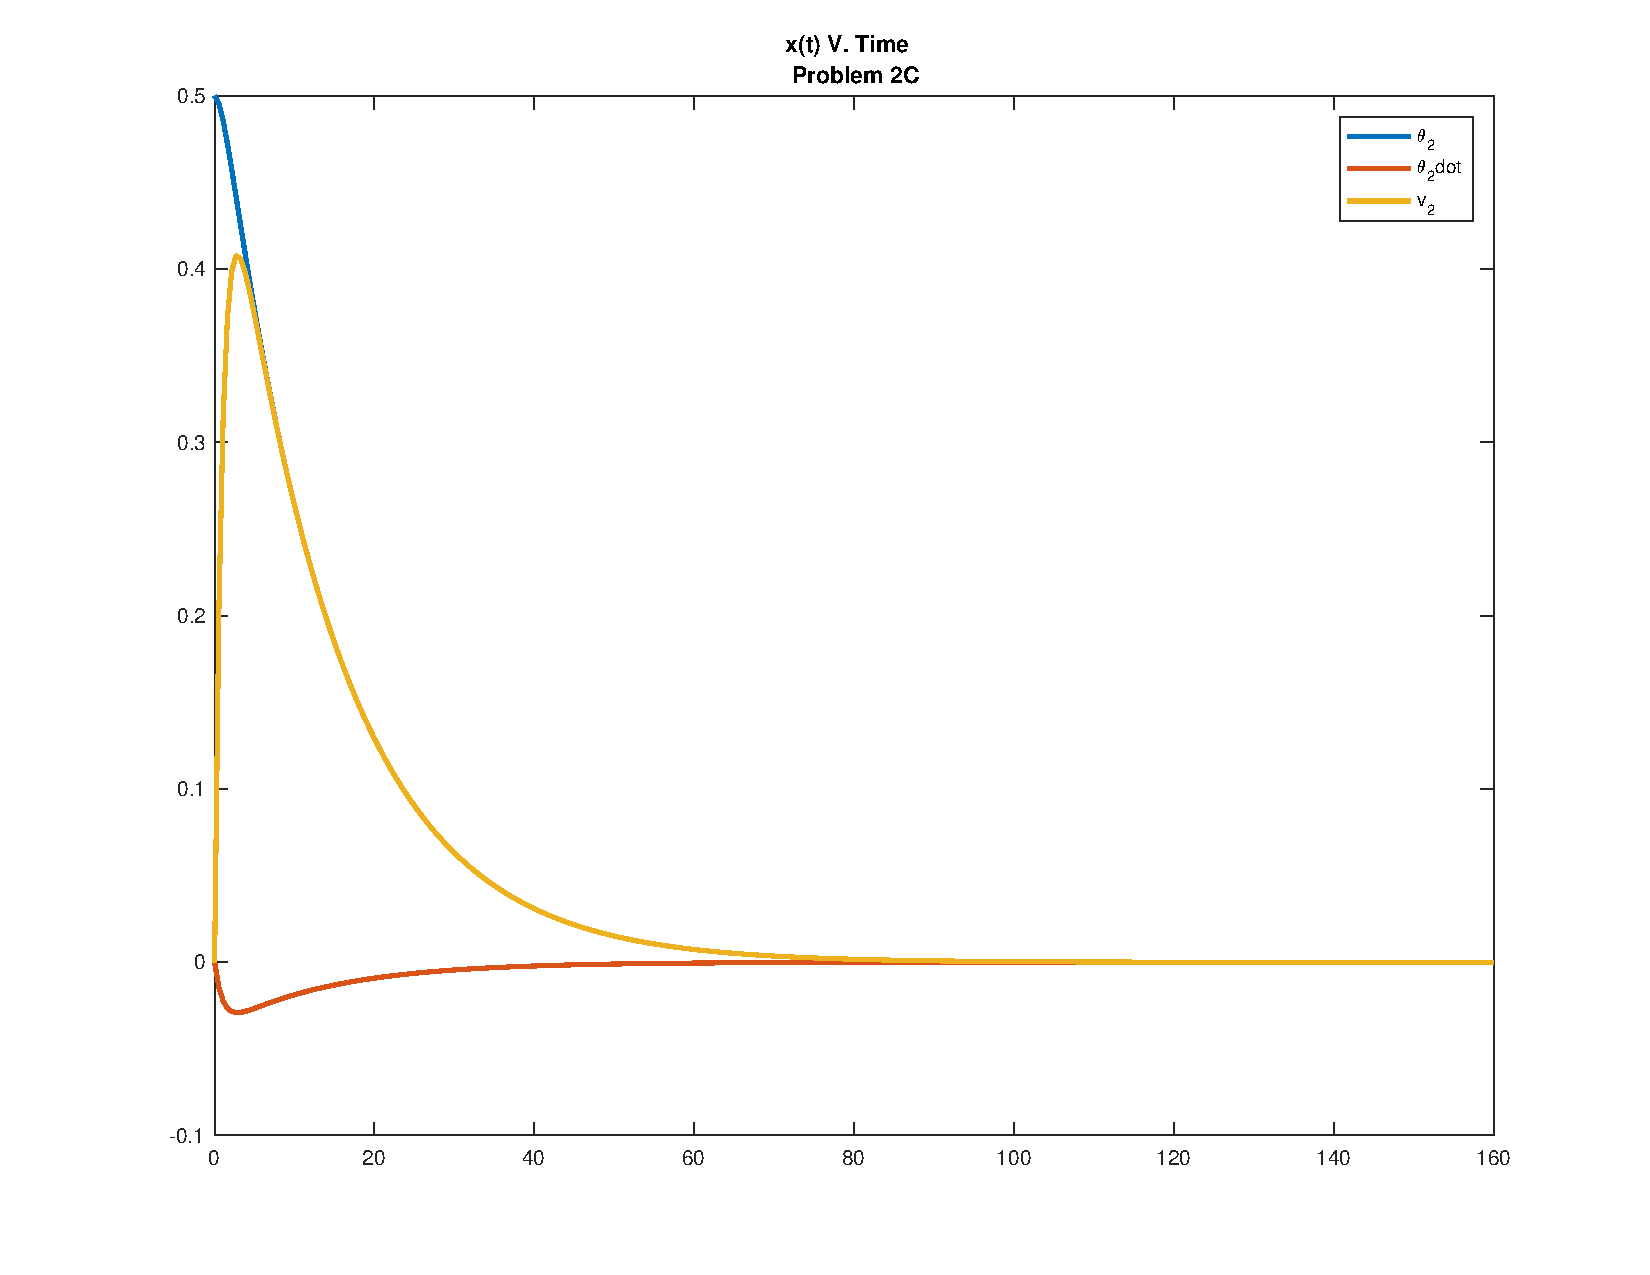
\includepdf{HW6P2C.pdf}

\begin{lstlisting}
function hw6p3
J1 = 12;
J2 = 14;
J3 = 8; 
Jw = 1; 
n = .0011;


A = [      0                 0               1               0          0     0;...
           0                 0               0               1          0     0;...
     -4*n^2*(J2-J3)/J1       0               0         n*(1-(J2-J3)/J1) 0     0;...
           0           n^2*(J1-J2)/J3 -n*(1+(J1-J2)/J3)      0          0     0;...
           0                 0               0               0          0     n;...
           0                 0               0               0         -n     0];
       
B = [0           0;...
     0           0;...
     1/J1        0;...
     0        1/J3;...
     -1/Jw       0;...
     0       -1/Jw];
 
x0 = [0.1 0.5 0 0 0 0]';

Q = eye(6);
R = 10^0.*eye(2); 

t = linspace(0,100,100);
% Part B
[k,s,e] = lqr(A,B,Q,R)

for i=1:length(t)
    x(:,i) = expm((A-B*k)*t(i))*x0;
end

%Superficial Plotting Code Hidden
figure(1) %x(t)
plot(t,x,'linewidth',2);
    
figure(2)
subplot(3,2,1)
plot(t,x(1,:),'linewidth',2);
subplot(3,2,3)
plot(t,x(2,:),'linewidth',2);
subplot(3,2,2)
plot(t,x(3,:),'linewidth',2);
subplot(3,2,4)
plot(t,x(4,:),'linewidth',2);
subplot(3,2,5)
plot(t,x(5,:),'linewidth',2);
subplot(3,2,6)
plot(t,x(6,:),'linewidth',2);

\end{lstlisting}
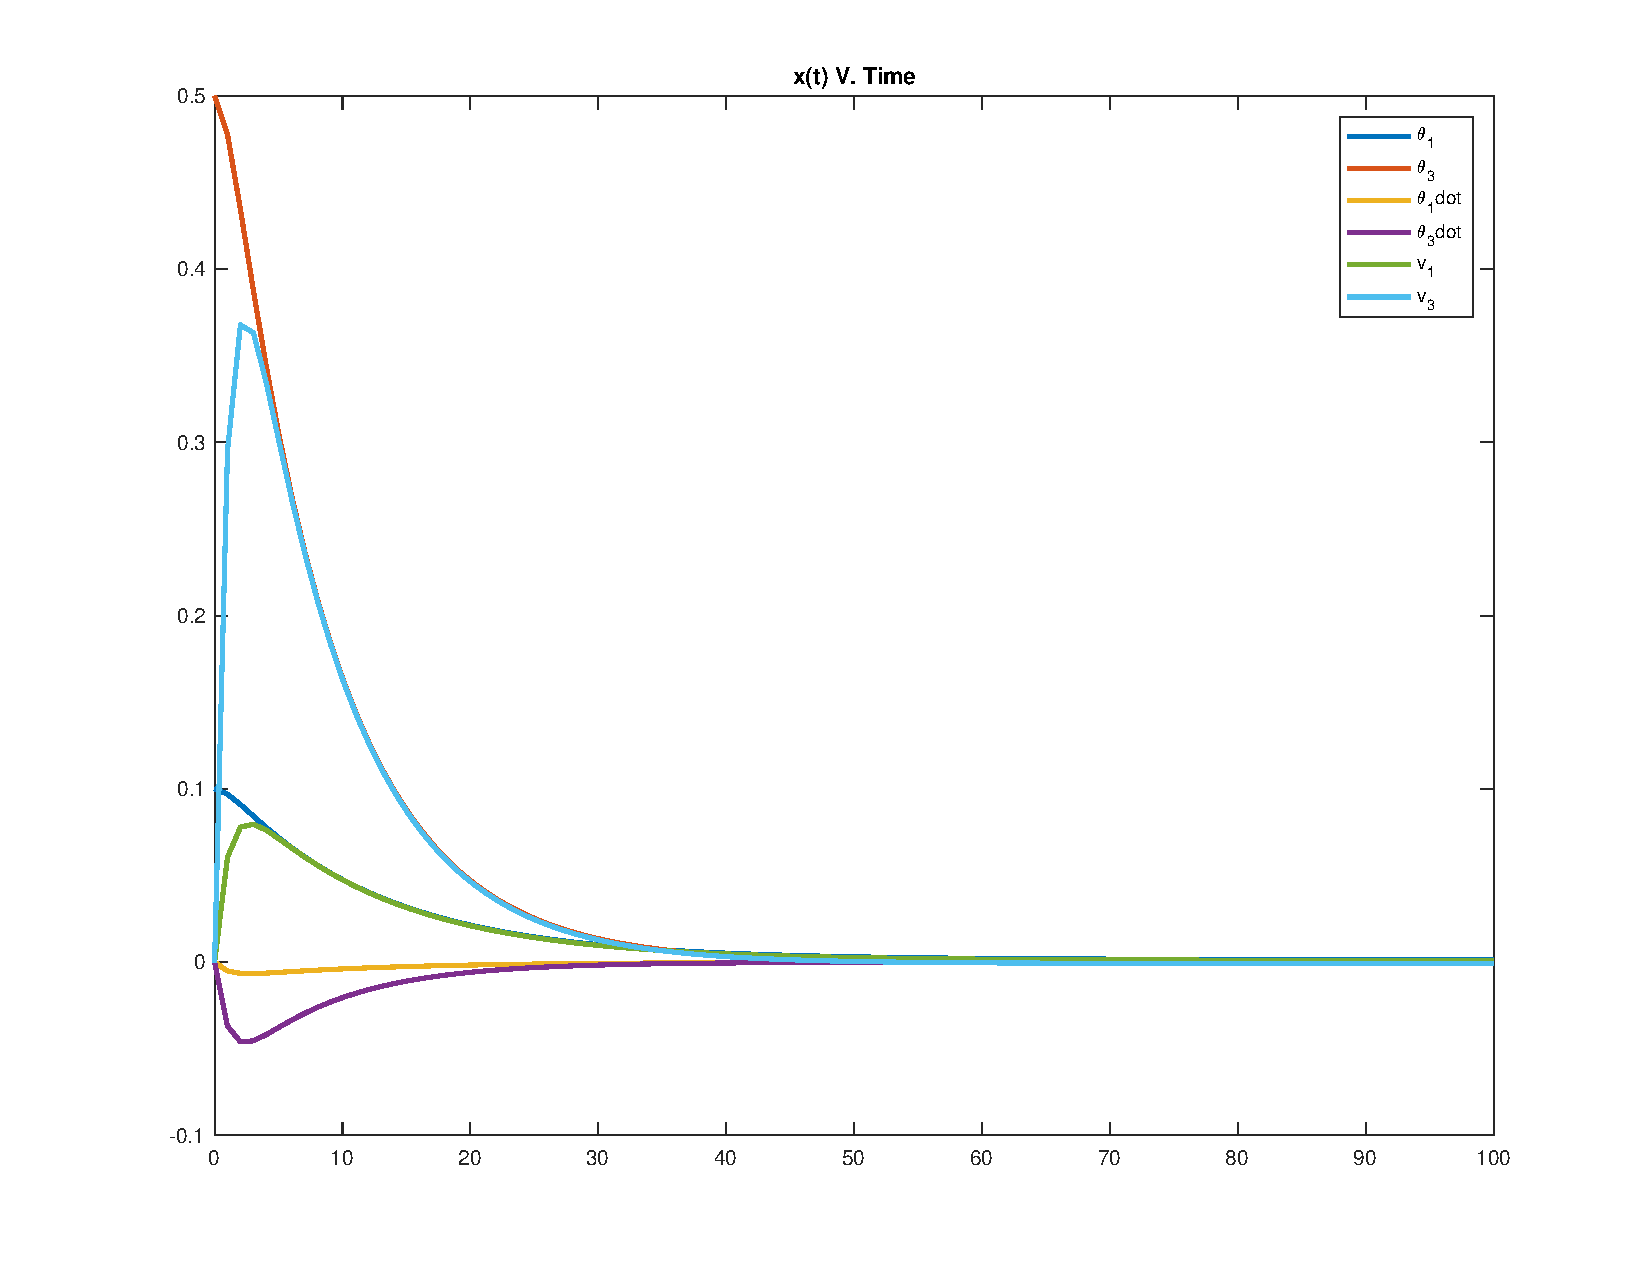
\includepdf{HW6P3C1.pdf}
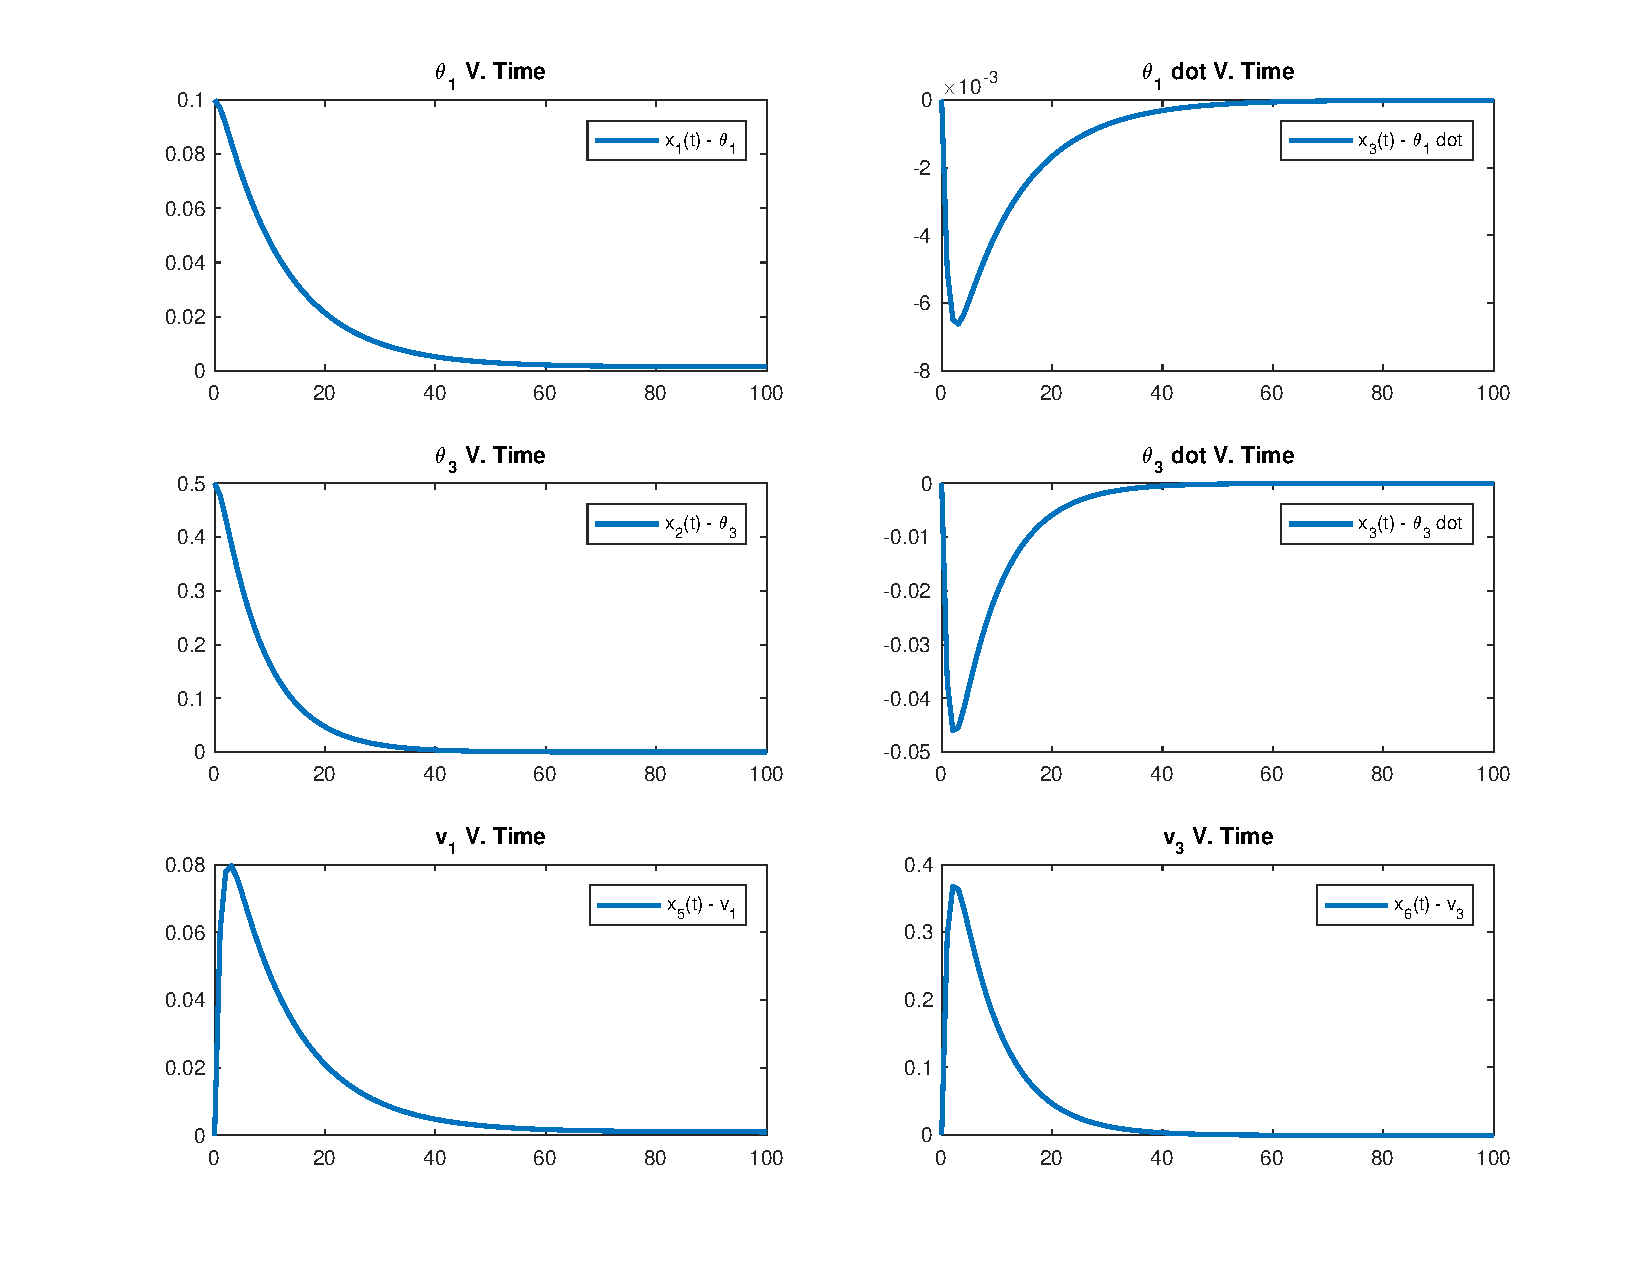
\includepdf{HW6P3C2.pdf}

\thispagestyle{empty}

\begin{center}
{\LARGE \bf Homework 6 Problem 4}\\
{\large AE403 - Spring 2018 \\ Emilio R. Gordon}
\end{center}
\vspace{0mm}
CUB-E is a $50cm\times50cm\times50cm$ nano-satellite with the scientific objective of deep-space astronomical observation. CUB-E orbits in low-earth orbit and has the attitude determination requirement of 10 arcsec and an attitude control requirement of 50arcsec over a 10-minute observation period. The target is inertially fixed but the craft is not. Since CUB-E is a nano-satellite, certain volumetric constraints lead to limitations and benefits to the ADCS. CUB-E will orbit in a near-polar, sun-synchronous orbit to allow for continuous solar cell charging and allowing the payload to remain focused on a fixed target without being blocked by the earth and having the payload constantly face away from the sun. 
\section*{Disturbances}
Orbiting in LEO leads to additional disturbances, especially on a craft this size. Perhaps the most limiting factor to CUB-E's attitude would be the \textbf{atmospheric drag} that often limits a nano-satellites lifetime. Aerodynamic Drag, also known as "Weathervane Effect" is due to an offset of the center of mass and the drag-center of pressure on the craft. Other disturbances that are typically considered are gravity gradient and solar radiation. \textbf{Gravity Gradient} is a "Tidal" Force due to  $\frac{1}{r^2}$ gravitational field variation over the length of the body of the craft. This is not a concern for CUB-E given its size and symmetrical shape (the lack of any booms or extensions).  \textbf{Solar radiation} can induce torques via the center of mass and center of pressure offset due to solar radiation on the body of the craft. For many of the same reasons of gravity gradient, this is not a concern for CUB-E. 
 
 An atypical disturbance that must be considered is internal torques caused by the payload. CUB-E's payload is a near-infrared telescope which must be kept at a cool temperature to minimize signal noise. As such, there is a possibility of having a cryocooler onboard which could have potential torque disturbances. These disturbances will have no net-effect but will have an internal moment exchange that does effect attitude.
\section*{Attitude Determination}
Given the tight requirements of this mission, a  \textbf{star tracker} is a necessary sensor since it has an accuracy of around 50sec. It would be beneficial to have two star-trackers for redundancy or improved accuracy. Each star tracker place on an opposite axis.

Another accurate attitude sensor to have on board would be a  \textbf{fiber-optic gyroscope} that senses changes in the orientation and returns the angular rate of the space-craft with an accuracy of $1.0 \times10^{-6} \, rad/s$. The FOG would ideally be placed along all three axis. With the star tracker and FOG, high accuracy for the attitude and angular rate can be determined. 

Alternative to the FOG would be a ring-laser gyroscope, which does not need to be calibrated and is less sensitive to vibrations (which should not be a problem onboard CUB-E given its size and lack of moving parts).

In addition, two sun-sensors should be equipped on each axis face, providing roughly 1degree of accuracy. Tthis will be beneficial for the periods of time before the star-tracker can provide the attitude. Finally, magnetometers and GPS can be implemented since CUB-E is in low-earth orbit, utilizing Earth's magnetic field and GPS network. These three can be implemented for initial attitude measurements that get fed as reference into the star tracker.
\section*{Attitude Control}
CUB-E will implement a 3-axis stabilization scheme that allows for accurate inertial reference pointing and requires active attitude control. This is a common spacecraft attitude scheme for communication and telescope satellites.  

Since CUB-E is a nano-satellite in LEO, magnetometers would be an ideal attitude control method. However, this posses a concern for the electronics aboard, especially the Star-tracker. Volumetric constraints due to the size prevent the magnetometer to be placed anywhere that would not pose a threat. Volumetric constraints also prevent any sort of thruster system to be used. 

The most reasonable control would be through reaction wheels along each of the three axis. An additional, skewed reaction wheel should be implemented for redundancy. With the reaction wheels onboard, the requirements for control are set. However, a source for momentum dumping must be made. At this point, the magnetometers can be used only for the case of momentum dumping. This, alongside proper placement, will allow for minimal interference of the magnetometer and the onboard electronics/star-tracker. 


\end{document}